\documentclass{article}
\usepackage{amsmath}
\usepackage{color}
\usepackage{tikz}
\usetikzlibrary{positioning}

\begin{document}

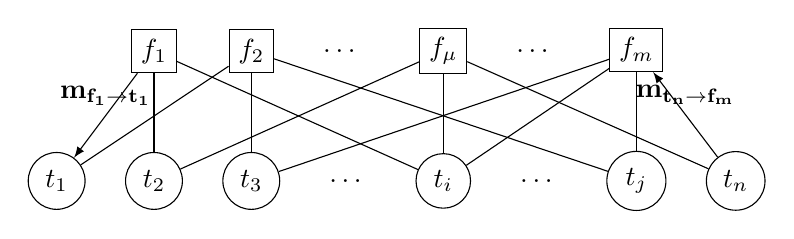
\begin{tikzpicture}[node distance=1.00cm and 0.5cm,>=latex, rotate=90]
	% Variables
	\node[draw, circle] (x1) {$t_1$};
	\node[draw, circle, right=of x1] (x2) {$t_2$};
	\node[draw, circle, right=of x2] (x3) {$t_3$};
	\node[right=of x3] (xdots1) {$\dots$};
	\node[draw, circle, right=of xdots1] (xi) {$t_i$};
	\node[right=of xi] (xdots) {$\dots$};
	\node[draw, circle, right=of xdots] (xn) {$t_j$};
	\node[draw, circle, right=of xn] (xnn) {$t_n$};

	% Factors
	\node[draw, rectangle, above=of x2] (f1) {$f_1$};
	\node[draw, rectangle, above=of x3] (f2) {$f_2$};
	\node[right=of f2] (fdots1) {$\dots$};
	\node[draw, rectangle, above=of xi] (f3) {$f_{\mu}$};
	\node[right=of f3] (fdots2) {$\dots$};
	\node[draw, rectangle, above=of xn] (fm) {$f_m$};

	% Connections and Messages
	\draw[->] (f1) -- (x1) node[midway, above] {$\mathbf{m_{f_1 \to t_1}}$};
	\draw[->] (xnn) -- (fm) node[midway, above] {$\mathbf{m_{t_n \to f_m}}$};

	% Connections
	\draw[-] (f1) -- (x2);
	\draw[-] (f1) -- (xi);
	\draw[-] (f2) -- (x1);
	\draw[-] (f2) -- (x3);
	\draw[-] (f2) -- (xn);
	\draw[-] (f3) -- (x2);
	\draw[-] (f3) -- (xi);
	\draw[-] (f3) -- (xnn);
	\draw[-] (fm) -- (x3);
	\draw[-] (fm) -- (xn);
	\draw[-] (fm) -- (xi);
\end{tikzpicture}

\end{document}